\documentclass[11pt,a4paper,oneside]{article}
\usepackage[dvipsnames, svgnames, x11names]{xcolor}
\usepackage{euler,amsthm,amsmath,amsfonts,graphicx,epigraph,indentfirst,enumerate,comment,listings,fontspec,color,subcaption,listings}
\usepackage{xeCJK}
\usepackage{hw}
\usepackage{pythonhighlight}
\usepackage{tikz}
\usepackage{algorithm}
\usepackage{algpseudocode}
\usepackage{float}

\newcommand{\nth}[1]{#1\textsuperscript{th}}
\newcommand{\E}{\mathop{\mathbb{E\/}}}


\renewcommand{\hwtitle} {CS217 Homework 2, First Submission}	
\renewcommand{\hwauthor}{Akina}
\renewcommand{\hwdate}{\today}

\begin{document}
\title{\hwtitle}
\author{\hwauthor}
\date{\hwdate}
\maketitle

\section*{Sorting Algorithms}
\begin{problem}{1}
	\statement
	Given an array $A$ of $n$ items (numbers), we can find the maximum with $n-1$ comparisons (this is simple).
	Show that this is optimal: that is, any algorithm that does $n-2$ or fewer comparisons will fail to find the maximum 
	on some inputs.
	\solution
	\begin{proof}
		Consider all the elements as vertices and comparisons as directed edges from larger to smaller ones, or the direction of the edge is arbitrary in the case of two elements are identical. Then consider how we conclude the maximum element: there's a path from the maximum element to every other element -- it's continuous inequations that mathematically proved the maximality.
		The simple algorithm forms a tree finally. Everytime it compares the current root and next element, adds an edge between them. Then the new root is decided according to the direction of the new edge.

		If there are $n - 2$ or fewer edges in the graph, the graph can not be connected since an edge can only decrease the number of connected components by 1. Howerver, in the beginning, we have $n$ components. What led to is that there are at least two components finally, which we don't really know their relations at all -- we can not conclude such inequation between any two vertices in different components, as well as the maximum element.
	\end{proof}
\end{problem}

\begin{problem}{2}
	\statement
	Let $A$ be an array of size $n$, where $n$ is even. 
	Describe how to find both the minimum and the maximum
	with at most $\frac{3}{2} n  - 2$ comparisons.
	Make sure your solution is {\em simple}, in describe it 
	in a clear and succinct way!

	\solution
	Life is short, I choose python.
\begin{python}
def min_max(a, n):
    small = []
    large = []
    for i in range(0, n, 2):
        res = a[i] > a[i + 1]
        small.append(a[i + res])
        large.append(a[i + 1 - res])
    return (min(small), max(large))
\end{python}
	First part, we make pair of every two ajancent number(their indexes are \(2n\) and \(2n + 1\) separately) and divides them by the result of comparisons which take $\frac n 2$ times.
	Second part we decide the maximum and minimum seperately, and both takes $\frac n 2 - 1$ comparisons(with use of the simple algorithm in Problem 1). In total, $\frac {3} {2} n - 2$ comparisons achieved.
\end{problem}
\begin{problem}{3}
	\statement
	Given an array $A$ of size $n = 2^k$, find the second largest element element
	with at most $n + \log_2(n)$ comparisons. 
	Again, your solution should be {\em simple}, and you should explain
	it in a clear and succinct way!
	
	\solution
	Life is even shorter, I choose python again.
\begin{python}
def second_max(a, n):
    b = [0] * (n + 1) + a
    for i in range(n - 1, 0, -1):
        b[i] = max(b[i * 2], b[i * 2 + 1])
    c = []
    x = 1
    while x < n:
        x *= 2
        x ^= b[x] != b[x >> 1]
        c.append(b[x ^ 1])
    return max(c)
\end{python}
	It's actually a segment tree. First part we do $n - 1$ comparisons to get the maximum element by a heap-like order, using an array of $2n$ elements to store the "comparison tree". In my implementation, to use $1$-indexed array there's an auxiliary number taking the place of $0$.
	
	\begin{figure}[H]
		\centering
		
		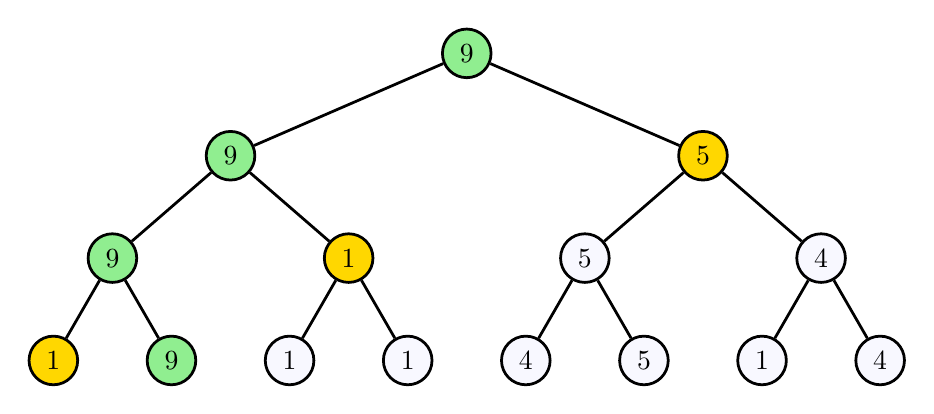
\begin{tikzpicture}[ grow'=down,
		 								line width = 1pt,
										vertex/.style={fill=none,draw,circle},
										level 1/.style={sibling distance=6cm, level distance=1.3cm},
										level 2/.style={sibling distance=3cm, level distance=1.3cm},
										level 3/.style={sibling distance=1.5cm, level distance=1.3cm}]
										
		\node [vertex, fill=LightGreen] {9}
			child {node[vertex, fill=Gold] {5}
				child {node[vertex, fill=GhostWhite] {4}
					child {node[vertex, fill=GhostWhite] {4}}
					child {node[vertex, fill=GhostWhite] {1}}
				}
				child {node[vertex, fill=GhostWhite] {5}
					child {node[vertex, fill=GhostWhite] {5}}
					child {node[vertex, fill=GhostWhite] {4}}
				}
			}
			child {node[vertex, fill=LightGreen] {9}
				child {node[vertex, fill=Gold] {1}
					child {node[vertex, fill=GhostWhite] {1}}
					child {node[vertex, fill=GhostWhite] {1}}
				}
				child {node[vertex, fill=LightGreen] {9}
					child {node[vertex, fill=LightGreen] {9}}
					child {node[vertex, fill=Gold] {1}}
				}
			};
		
		\end{tikzpicture}
		\caption{An example of $[1, 9, 1, 1, 4, 5, 1, 4]$}
	\end{figure}

	Now get back and see how the maximum is elected: each root of subtree is the maximum of 
	all leaves corresponding to an interval of the original sequence. The path which 
	indicates how root is elected is marked in green, and the sibling nodes of the path are marked in yellow.
	It's easy to show that the second maximum is maximum of yellow nodes, since the second maximum is the maximum of all elements except the maximum,
	and the yellow node contains all infomation about the maximum of other elements.
	The number of yellow nodes is $\log_2(n) - 1$ since the height of the tree is $\log_2{n}$, so the second step consumes $\log_2(n) - 2$ comparisons.

	In total, $n + \log_2(n) - 2$ comparisons achieved.
\end{problem}

\section*{Quickselect}

Remember the recursive algorithm \textsc{QuickSelect} from the lecture. I write
it below in pseudocode. In analogy to quicksort we define QuickSelect deterministically
and assume that the input array is random, or has been randomly shuffled before
QuickSelect is called. We assume that $A$ consists of distinct elements and
$1 \leq k \leq |A|$.

Let $C$ be the number of comparison made by $\textsc{QuickSelect}$. In the 
lecture we proved that $\E[C] \leq O(n)$ when we run it on a random input.

\begin{problem}{5}
\statement
Explain how \textsc{QuickSelect} can be viewed as a "partial execution'' of quicksort
with the random pivot selection rule.
Draw an example quicksort tree and show which part of this tree is visited
by \text{QuickSelect}.

\begin{algorithm}
	\caption{Select the \nth{$k$} smallest element from a list $A$}
	\begin{algorithmic}[1]
		\Procedure{QuickSelect}{$X,k$}
		\If{$|X| = 1$}
		\State \Return $X[1]$
		\Else:
		\State $p := X[1]$
		\State $Y:= [ x \in X \ | \ x < p]$
		\State $Z := [ x \in X \ | \ x > p]$
		\If{$|Y| = k-1$}
		\State \Return $p$
		\ElsIf{$|Y| \geq k$}
		\State \Return $\textsc{QuickSelect}(Y,k)$
		\Else
		\State Return $\textsc{QuickSelect}(Z, k- |Y| - 1)$
		\EndIf
		\EndIf
		\EndProcedure
	\end{algorithmic}
\end{algorithm}

\solution

We explain by example. Here's a quicksort tree for sorting \(A = \left \{ 2, 9, 6, 7, 1, 10, 5, 4, 8, 3\right \}\)

\begin{figure}[H]
	\centering
	
	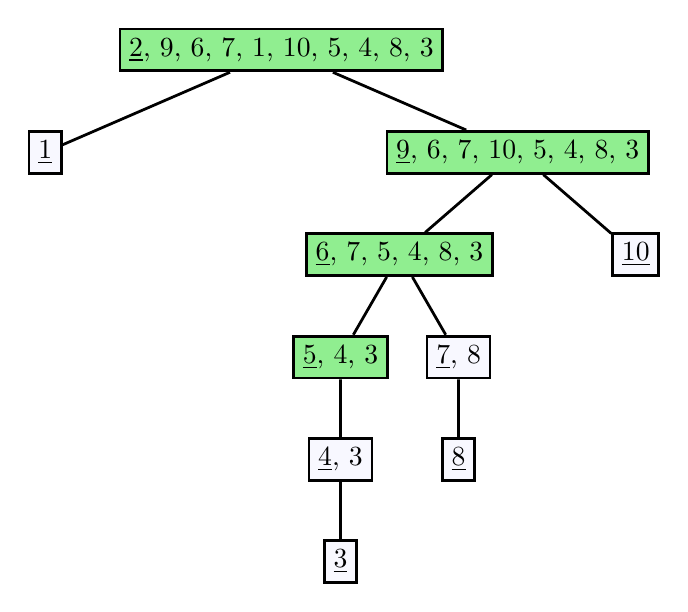
\begin{tikzpicture}[ grow'=down,
	line width = 1pt,
	vertex/.style={fill=none,draw,rectangle},
	level 1/.style={sibling distance=6cm, level distance=1.3cm},
	level 2/.style={sibling distance=3cm, level distance=1.3cm},
	level 3/.style={sibling distance=1.5cm, level distance=1.3cm}]
	
	\node [vertex, fill=LightGreen] {\underline{2}, 9, 6, 7, 1, 10, 5, 4, 8, 3}
		child {node[vertex, fill=LightGreen] {\underline{9}, 6, 7, 10, 5, 4, 8, 3}
			child {node[vertex, fill=GhostWhite] {\underline{10}}}
			child {node[vertex, fill=LightGreen] {\underline{6}, 7, 5, 4, 8, 3}
				child {node[vertex, fill=GhostWhite] {\underline{7}, 8}
					child {node[vertex, fill=GhostWhite] {\underline{8}}}
				}
				child {node[vertex, fill=LightGreen] {\underline{5}, 4, 3}
					child {node[vertex, fill=GhostWhite] {\underline{4}, 3}
						child {node[vertex, fill=GhostWhite] {\underline{3}}}
					}
				}
			}
		}
		child {node[vertex, fill=GhostWhite] {\underline{1}}};
		
	
	\end{tikzpicture}
	\caption{Quickselect \nth{\(5\)} in quicksort tree for \(\left \{ 2, 9, 6, 7, 1, 10, 5, 4, 8, 3\right \}\)}
\end{figure}

QuickSelect is quite similar to QuickSort. They both select the first element as the pivot and divide the set into two subsets. What different is that QuickSelect Algorithm do recursion only for one part(i.e. either the part greater than the pivot or the part less than the pivot). If we want to find the \nth{\(5\)} element in the above example, we only need to visit the node filled in green in the quicksort tree.

That's why QuickSelect can be viewed as a "partial execution'' of quicksort.

\end{problem}

\begin{problem}{6}
\statement
Let $B_{i,j,k}$ be an indicator variable which is $1$ if $i$ is a common ancestor
of $j$ and $k$ in the quicksort tree. That is, if both $j$ and $k$ appear in the 
subtree of $T(\pi)$ rooted at $i$.

What is $\E[B_{i,j,k}]$? Give a succinct formula for this.

\solution
\begin{lemma}
	$B_{i, j, k} = 1$ if and only if $i$ comes earlier than any element in $[\min(i, j, k), \max(i, j, k)]$

	\begin{proof}
		We proved that \(A_{i, j} = 1\) if and only if \(i\) comes first in \([\min(i, j), \max(i, j)]\). Express B using A, we got 
		$$B_{i, j, k} = A_{i, j}A_{i, k}$$ 
		Thus \(i\) comes first than any other element in $[\min(i, j, k), \max(i, j, k)]$
	\end{proof}
	
\end{lemma}

Hence,

\[ B_{i, j, k} = \frac{1}{\max(i, j, k) - \min(i, j, k) + 1} \]
\end{problem}

\begin{problem}{7}
\statement
Let $C(\pi,k)$ be the number of comparisons made by \textsc{QuickSelect} when given
$\pi$ as input. Design a formula for $C(\pi,k)$ with the help of the indicator
variables $A_{i,j}$ and $B_{i,j,k}$ (analogous to the formula 
$\sum_{i \ne j} A_{i,j}$ for the number of comparisons made by quicksort).

\solution
\begin{lemma}
$$C(\pi,k)=\sum_{i \ne k} A_{i,k}+\sum_{i \ne k} A_{k,i}+\sum_{i \ne j,i \ne k,j\ne k} B_{i,j,k}$$
\end{lemma}
\begin{proof}

For an element $i$ different from $k$, there're $3$ cases for it:
\begin{itemize}
	\item Becoming a pivot before found $k$, i.e. $A_{i, k} = 1$
	\item Still in the same part with $k$ when $k$ is chosen as pivot, i.e. $A_{k, i} = 1$
	\item Been ``thrown away'' since it was divided into another part by some pivot, i.e. $A_{i, k} + A_{k, i} = 0$
\end{itemize}

Count seperately, we have
\begin{itemize}
	\item $A_{i, k} (1 + \sum_{j \neq i} A_{j, i}) = A_{i, k} (1 + \sum_{j \neq i, j \neq k} B_{j, i, k})$
	\item $A_{k, i} (1 + \sum_{j \neq k} A_{j, k}) = A_{k, i} (1 + \sum_{j \neq i, j \neq k} B_{j, i, k})$
	\item $(1 - A_{k, i} - A_{i, k})(\sum_{j \neq i, j \neq k} B_{j, i, k})$
\end{itemize}

In total,
\begin{align*}
	C(\pi,k) &= \sum_{i \neq k} (A_{i, k} (1 + \sum_{j \neq i, j \neq k} B_{j, i, k}) +A_{k, i} (1 + \sum_{j \neq i, j \neq k} B_{j, i, k}) +(1 - A_{k, i} - A_{i, k})\sum_{j \neq i, j \neq k} B_{j, i, k}) \\
	&= \sum_{i \ne k} A_{i,k}+\sum_{i \ne k} A_{k,i}+\sum_{i \ne j,i \ne k,j\ne k} B_{i,j,k}
\end{align*}

\end{proof}
\end{problem}


\begin{problem}{8}
\statement
Suppose we use \textsc{QuickSelect} to find the minimum of the array. On expectation,
how many comparisons will it make? Give an answer that is exact up to additive terms 
of order $o(n)$.
You can use the fact that $H_n := 1 + \frac{1}{2} + \frac{1}{3} + \cdots  + \frac{1}{n} = \ln(n) + o(1)$.
\solution
\begin{proof}
	We have found a formula for $C(\pi,k)$ in the last problem. Therefore we only need to calculate $\E[C(\pi,1)]$.

	(See next page)

    \[
        \begin{split}
            \E[C(\pi,1)] &= \E[\sum_{i \not= 1}A_{i, 1} + \sum_{i \not= 1}A_{1, i} + \sum_{i \not= j, i \not= 1,j \not= 1}B_{i, j, 1}]\\
            &= \E[\sum_{i \not= 1}A_{i, 1} + \sum_{i \not= 1}A_{1, i} + \sum_{2 \leq i < j \leq n}B_{i, j, 1} + \sum_{2 \leq j < i \leq n}B_{i, j, 1}]\\
            &= \sum_{i \not= 1} \E[A_{i, 1}] + \sum_{i \not= 1} \E[A_{1, i}] + \sum_{2 \leq i < j \leq n}\E[B_{i, j, 1}] + \sum_{2 \leq j < i \leq n}\E[B_{i, j, 1}]\\
            &= \sum_{i \not= 1} \frac{1}{i} + \sum_{i \not= 1} \frac{1}{i} + \sum_{2 \leq i < j \leq n} \frac{1}{j} + \sum_{2 \leq j < i \leq n}\frac{1}{i}\\
            &= \sum_{i \not= 1} \frac{1}{i} + \sum_{i \not= 1} \frac{1}{i} + \sum_{2 < j \leq n}(1 - \frac{2}{j}) + \sum_{2 < i \leq n}(1 - \frac{2}{i})\\
            &= (H_n - 1) + (H_n - 1) + (n - 2) - 2(Hn - \frac{3}{2}) + (n - 2) - 2(Hn - \frac{3}{2})\\
            &= 2n + O(\ln n)
        \end{split}
    \]
    Thus, $2n + O(n)$ comparisons are made on expectation.
\end{proof}
\end{problem}

\begin{problem}{9}
\statement
Derive a formula for $\E_{\pi} [C(\pi,k)]$, up to additive terms of order $o(n)$.
You might want to introduce $\kappa := k/n$.

\solution
(See next page)
\begin{proof}
    \[
        \begin{split}
            \E_{\pi} [C(\pi,k)] &= \E[\sum_{i \not= k}A_{i, k} + \sum_{i \not= k}A_{k, i} + \sum_{i \not= j, i \not= k,j \not= k}B_{i, j, k}]\\
            &= \sum_{i \not= k}\E[A_{i, k}] + \sum_{i \not= k}\E[A_{k, i}] + \sum_{i \not= j, i \not= k,j \not= k}\E[B_{i, j, k}]\\\\
            \sum_{i \not= k}\E[A_{i, k}] + \sum_{i \not= k}\E[A_{k, i}] &= 2\sum_{i \not= k}\frac{1}{|i - k| + 1} \\
            &= 2(H_k + H_{n - k + 1} - 2)\\\\
            \sum_{i \not= j, i \not= k,j \not= k}\E[B_{i, j, k}] &= (\sum_{i < j < k} + \sum_{j < i < k} + \sum_{k < i < j} + \sum_{k < j < i} + \sum_{i < k < j} + \sum_{j < k < i}) \E[B_{i, j, k}] \\\\
            (\sum_{i < j < k} + \sum_{j < i < k})\E[B_{i, j, k}] &= \sum_{i < j < k}\frac{1}{k - i + 1} + \sum_{j < i < k}\frac{1}{k - j + 1}\\
            &= \sum_{1 \leq i < k - 1}1 - \frac{2}{k - i + 1} + \sum_{1 \leq j < k - 1} 1 - \frac{2}{k - j + 1}\\
            &= 2k - 4H_k + 2\\\\
            (\sum_{k < i < j} + \sum_{k < j < i})\E[B_{i, j, k}] &= \sum_{k < i < j}\frac{1}{j - k + 1} + \sum_{k < j < i}\frac{1}{i - k + 1}\\
            &= \sum_{k + 1 < j \leq n}1 - \frac{2}{j - k + 1} + \sum_{k + 1 < i \leq n} 1 - \frac{2}{i - k + 1}\\
            &= 2(n - k) - 4(H_{n - k + 1} - 1)\\
            &= 2(n - k + 1) - 4H_{n - k + 1} + 2\\\\
            (\sum_{i < k < j} + \sum_{j < k < i}) \E[B_{i, j, k}] &= \sum_{i < k < j}\frac{1}{j - i + 1} + \sum_{j < k < i}\frac{1}{i - j + 1} \\
            &= 2(\sum_{1 \leq i < j \leq n}\frac{1}{j - i + 1} - \sum_{1 \leq i < j \leq k}\frac{1}{j - i + 1} - \sum_{k \leq i < j \leq n}\frac{1}{j - i + 1})\\
            &= 2(((n + 1)H_n -2n) - ((k + 1)H_k -2k) - ((n - k + 1 + 1)H_{n - k + 1} - 2(n - k + 1)))\\
            &= (2n + 2)H_n - (2k + 2)H_k - (2n - 2k + 4)H_{n - k + 1} + 4\\\\
            \E_{\pi} [C(\pi,k)] &= (2n + 2)H_n - (2k + 4)H_k - (2n - 2k + 6)H_{n - k + 1} + 2n + 6\\
            &= ((2n + 2) - (2k + 4)\frac{H_k}{H_n} - (2n - 2k + 6)\frac{H_{n - k + 1}}{H_n})H_n + 2n + 6\\
            &\leq ((2n + 2) - (2k + 4)\kappa - (2n - 2k + 6)(1 - \kappa))H_{n} + 2n + 6 \\
            &= (2\kappa(1 - \kappa)n + 2\kappa - 4)(H_n) + 2n + 6\\
            &= 2\kappa(1 - \kappa)n\log_2(n) + 2n + O(n)
        \end{split}
    \]
\end{proof}
\end{problem}
\end{document}
